\chapter{The Relativistic Heavy Ion Collider}

\section{Overview}
While there have been many experiments which have performed deep inelastic
scattering over the years, the experiments built around the Relativistic Heavy
Ion Collider at Brookhaven National Laboratory are positioned to take advantage
of the unique accelerator. 

\begin{figure}[ht]
  \centering
  \begin{subfigure}[b]{\textwidth}
    \centering
    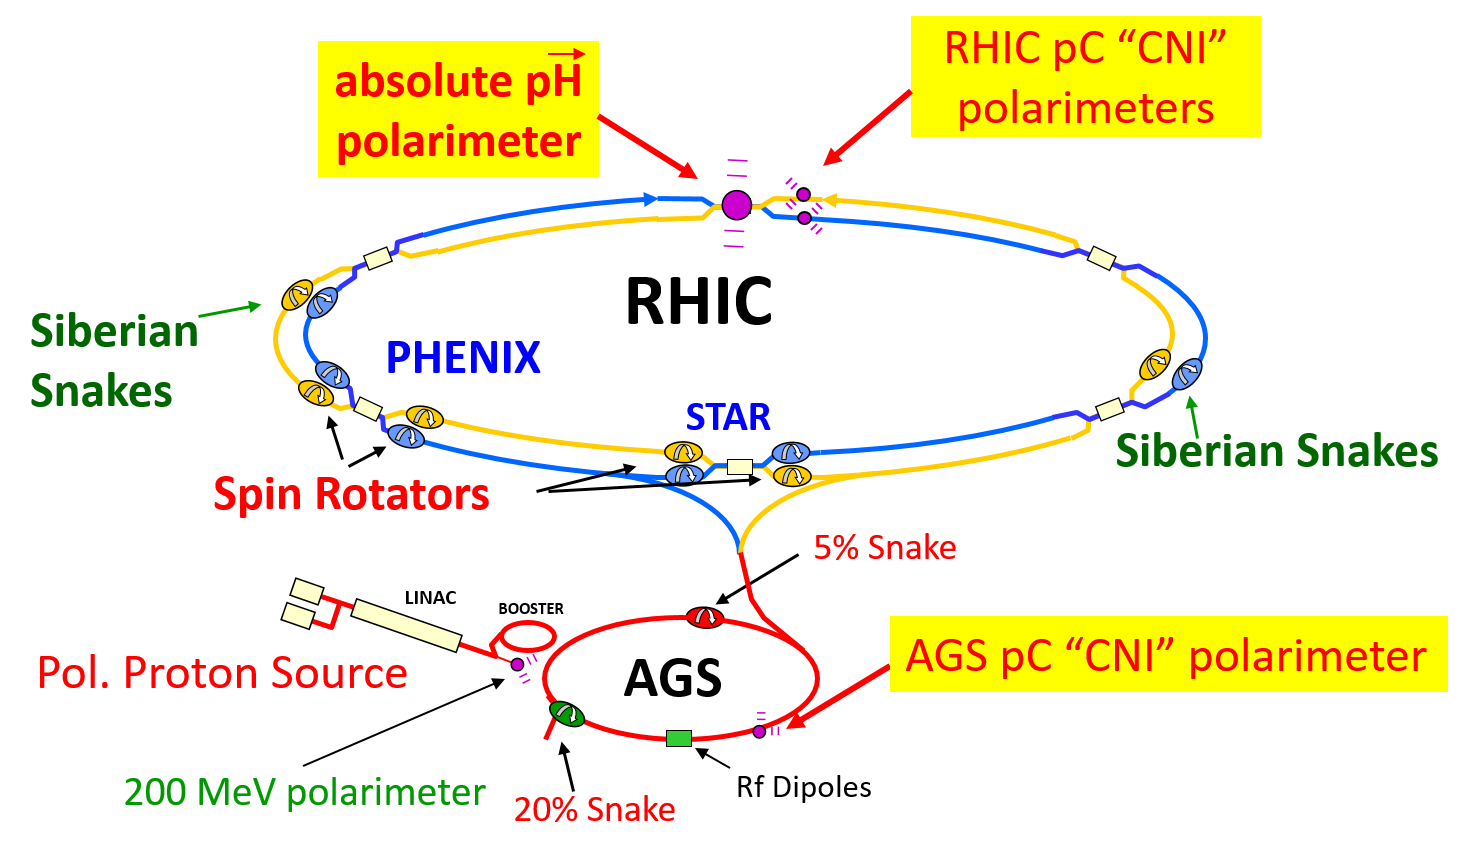
\includegraphics[width=0.8\linewidth]{figures/kiyoshi_tanida_rhic_schematic.png}
    \caption{Diagram of RHIC Accelerator Complex, (Figure from Kiyoshi Tanida)}
    \label{fig:rhic_schematic} 
  \end{subfigure}
  \begin{subfigure}[b]{\textwidth}
    \centering
    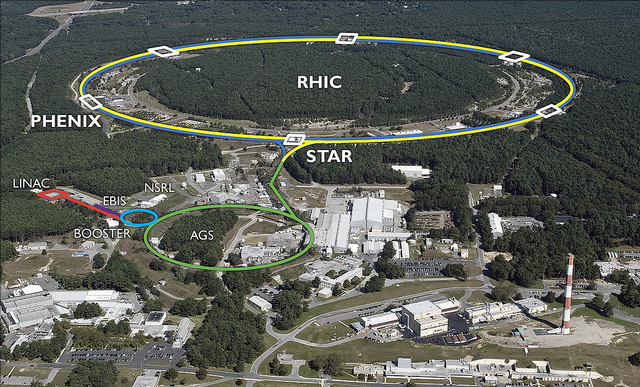
\includegraphics[width=0.8\linewidth]{figures/7979381212_fddf3f1ab4_z.jpg}
    \caption{Aerial photograph of RHIC Complex \cite{BNLFlickr2011}}
    \label{fig:rhic_aerial}
  \end{subfigure}
  \caption{
    A diagram of the acceleration process of RHIC is shown in the top panel, and
    aerial view is on bottom. RHIC is nearly four miles in circumference and
    collides a variety of ions at center-of-mass energies between $62 GeV$ and
    $510 GeV$.
  }
  \label{fig:rhic_complex}
\end{figure}

The Relativistic Heavy Ion Collider (RHIC) is the world's only intersecting ring
particle accelerator which is capable of producing polarized proton beams. The
beams are differentiated with the mnemonic "Blue" and "Yellow" beam. The Blue
beam circulates clockwise when viewed from above the RHIC complex, the Yellow
beam circulates counter-clockwise. As is typical for intersecting ring
experiments, the beams are bunched, with bunches of ions intersecting at
designated intersection points, around which experiments are built. The Blue
beam is nominally used to time these collisions, such that experiments which
have bunch-sensitive measurements (i.e. any experiment where bunch polarization
is important) can associate the correct punch polarization with the correct
collision. This will be discussed more in the section of beam-polarization
(\ref{sec:beam_polarization}).

Scientists at RHIC have come up with many ingenious ways to create and maintain
beam polarization, once this is accomplished, various kinematically select
probes are engineered, based on collisions observed which provide important
cross-checks to DIS data as well as original discoveries and measurements of
proton structure. RHIC is a unique collider in that it is quite flexible. Beams
may be transversely or longitudinally polarized, a variety of ions may be used
to fill the beams. To date, RHIC has collided many beam ions and species,
summarized in Figure~\ref{fig:rhic_early_run_summary} and
Figure~\ref{fig:rhic_late_run_summary}.

\begin{figure}[ht]
  \centering
  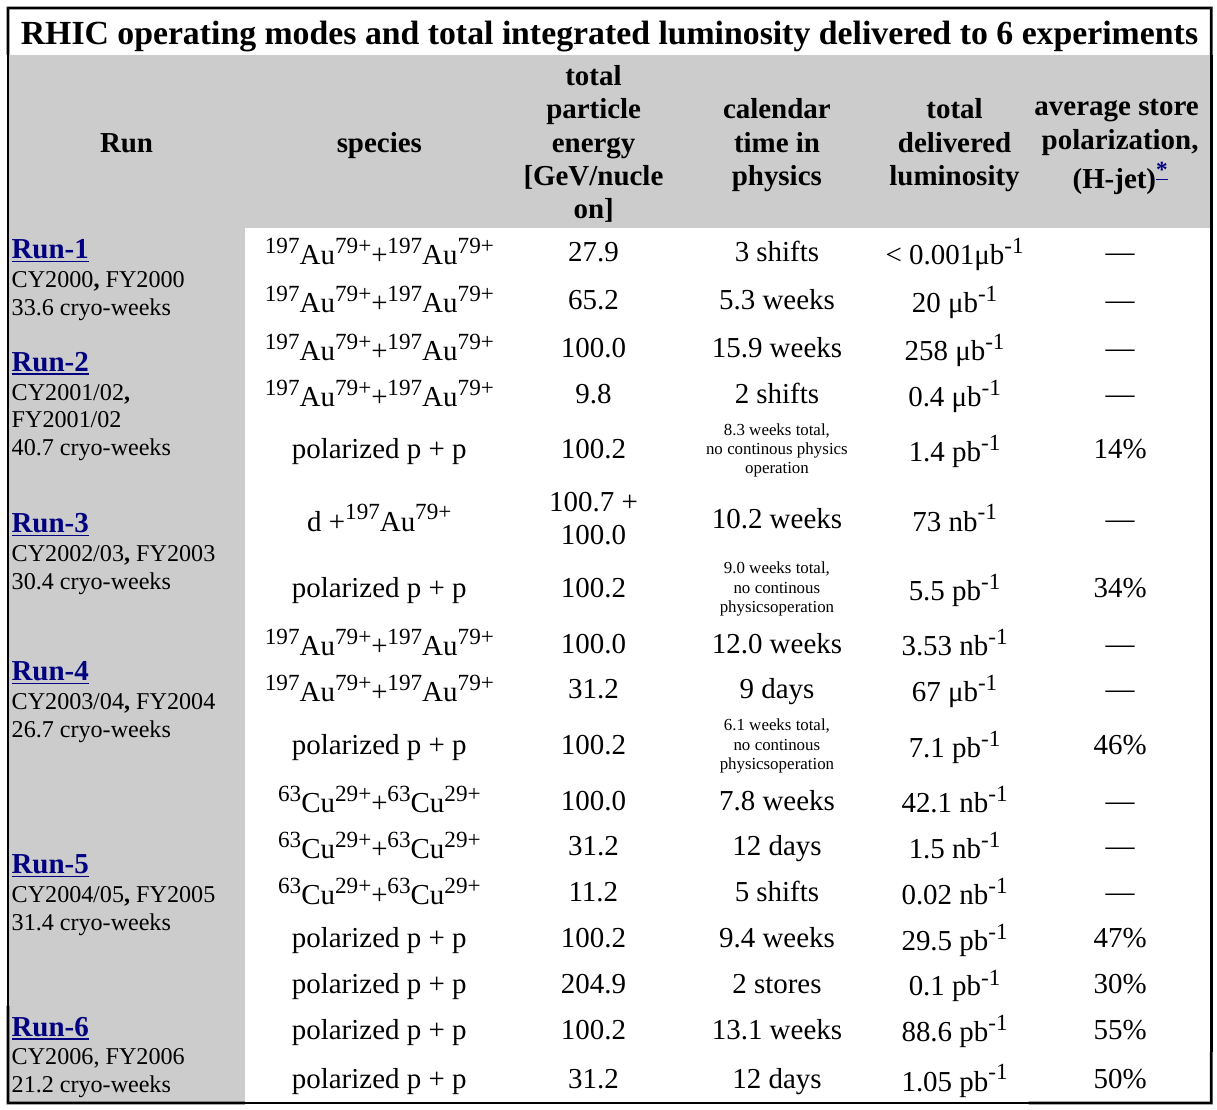
\includegraphics[width=0.8\linewidth]{figures/rhic_early_run_summary.png}
  \caption{ 
    Runs 1 - 3 at RHIC focused on commissioning work for experiments measuring
    collisions at RHIC. Work was mostly characterized by heavy-ion measurements
    related to understanding Quark-Gluon Plasma. The spin program began with Run
    5. Table produced from data posted at the RHIC run page \cite{Fischer2016}.
  }
  \label{fig:rhic_early_run_summary}
\end{figure}

\begin{figure}[ht]
  \centering
  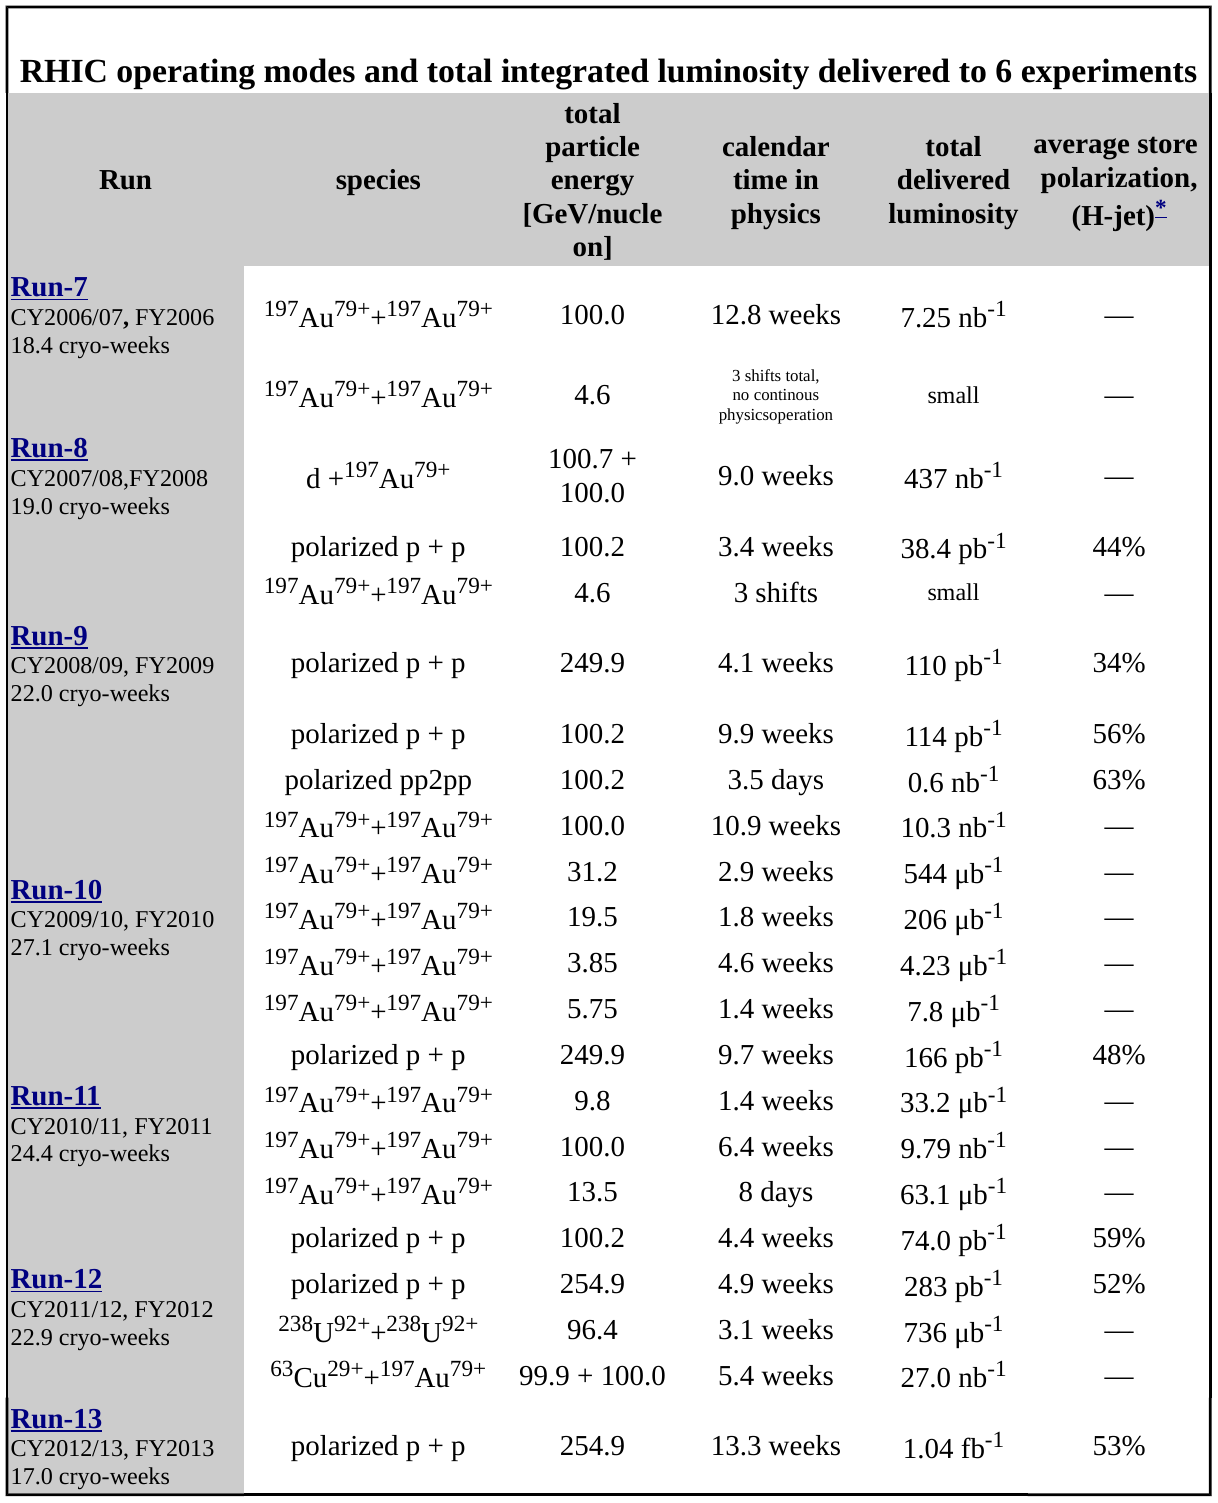
\includegraphics[width=0.8\linewidth]{figures/rhic_late_run_summary.png}
  \caption{ 
    Though RHIC is currently still running (as of May 9, 2016), I include runs
    here up to and including the run producing my data set (Run 13). An
    unprecedented 13.3 cryo-weeks of running was awarded to the W-Physics
    group.  Table produced from data posted at the RHIC run
    page \cite{Fischer2016}.
  }
  \label{fig:rhic_late_run_summary}
\end{figure}

At the time of writing of this thesis (Spring of 2016), there are two
experiments which are actively taking data from collisions produced by RHIC: The
Pioneering High Energy Nuclear Interaction Experiment (PHENIX,
Section~\ref{sec:PHENIX}, Figure~\ref{fig:phenix_and_star}), and the Solenoidal
Tracker at RHIC (STAR, Figure~\ref{fig:phenix_and_star}). STAR and PHENIX are
complimentary to each other - PHENIX has a very high precision centrally
covering Electromagnetic Calorimeter, and other high precision detectors, but
lacks full kinematic coverage, whereas STAR has lower precision, but has nearly
full kinematic coverage around the beam intersection at its center.

RHIC's luminosity and beam polarization has been continuously improving
(Figure~\ref{fig:rhic_luminosity}) since RHIC was first turned on. As we will
discuss later (\ref{sec:forward_upgrade}), this increased luminosity observed in
2013, was maximally leveraged with upgrades to the PHENIX detector.

\begin{figure}[ht]
  \centering
  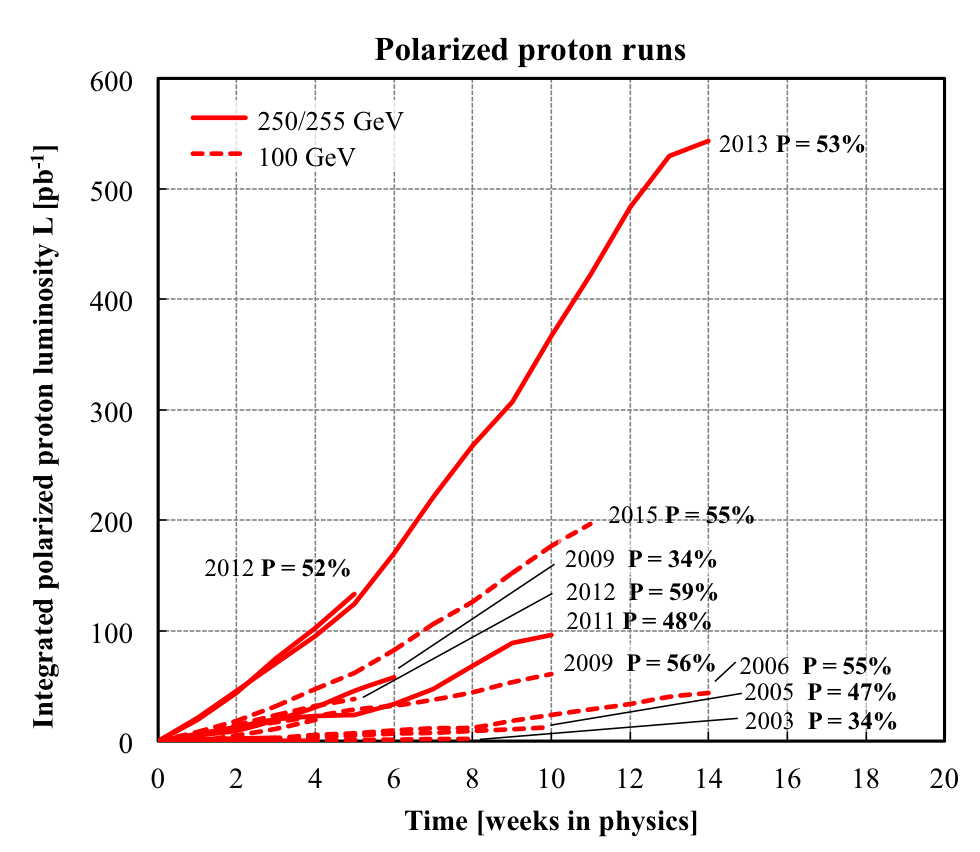
\includegraphics[width=0.8\linewidth]{figures/RhicLuminosityPP.png}
  \caption{
    Upgrades to RHIC's electron lens have enabled massive improvements to
    luminosity - seen in the year 2013. The high luminosity was taken advantage
    of with an extra long proton+proton run. Figure obtained from
     \cite{Fischer2016}
  }
  \label{fig:rhic_luminosity}
\end{figure}


\clearpage

\subsection{Experimental Apparatus}

\begin{figure}[ht]
  \centering
  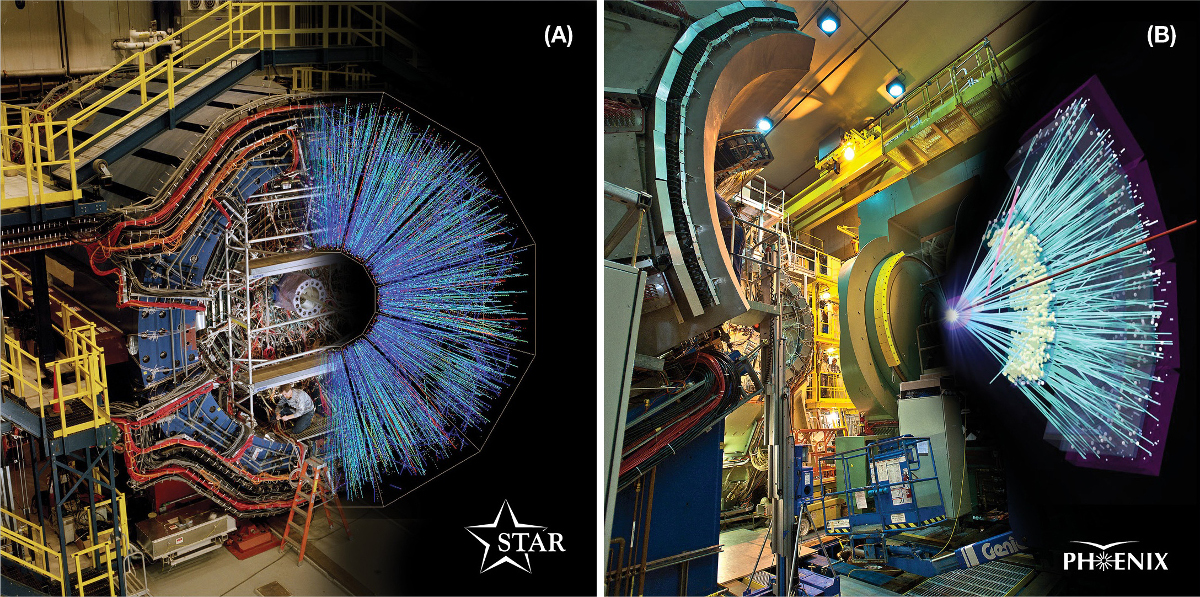
\includegraphics[width=\linewidth]{figures/rhic_graphics_fig2-hr.jpg}
  \caption{
    STAR (a) and PHENIX (b) with cutaways showing the event display for a
    heavy-ion collision as reconstructed by the detectors' electromagnetic
    calorimeters~\cite{Walsh2012}.
  }
  \label{fig:phenix_and_star}
\end{figure}

RHIC accelerates ions in a multi-stage process, summarized in
Figure~\ref{fig:rhic_complex}. The first stop is the \textbf{Electron Beam Ion
Source}, built on top of a $200 MeV$ linear accelerator (Linac). Once ions are
injected into the Linac, they travel to the $Booster Synchrotron$.  At this
stage, ions are accelerated with pulsed RF fields. Once the beam of ions has
been accelerated to nearly the speed of light, they are fed into the
\textbf{Alternating Gradient Synchrotron} or AGS. At this time, ions are
traveling at about 0.37~$c$. By the time the ions leave the AGS, they are moving
at 0.997~$c$. Once the ions are ready, they are transferred to the
\textbf{AGS-to-RHIC Line}, where a switching magnet pumps bunches of ions into
either the counterclockwise circulating ring of RHIC, or the clockwise
circulating ring of RHIC. The ions are 'spun-up' here to maximum speed, and are
accelerated around the RHIC complex - each beam-ion travels nearly 2.4 miles in
microseconds, for the duration of a physics-fill~\cite{RHIC2016}.

When the RHIC rings are filled with ions, the ions are bunched into rotating
electromagnetic potentials called 'buckets'. There are 360 beam-buckets in
total, but typically only a fraction are filled with ions. For this analysis, we
took data with beams with 110 filled buckets. The sequence of beam buckets from
one bunch to the next is referred to as a 'bunch' - and are rather long -
Figure~\ref{fig:bunch_profile_overlay}. A detailed presentation of beam dynamics
with regards to luminosity will be presented in chapter
\ref{ch:vernier_analysis}.

\begin{figure}
  \centering
  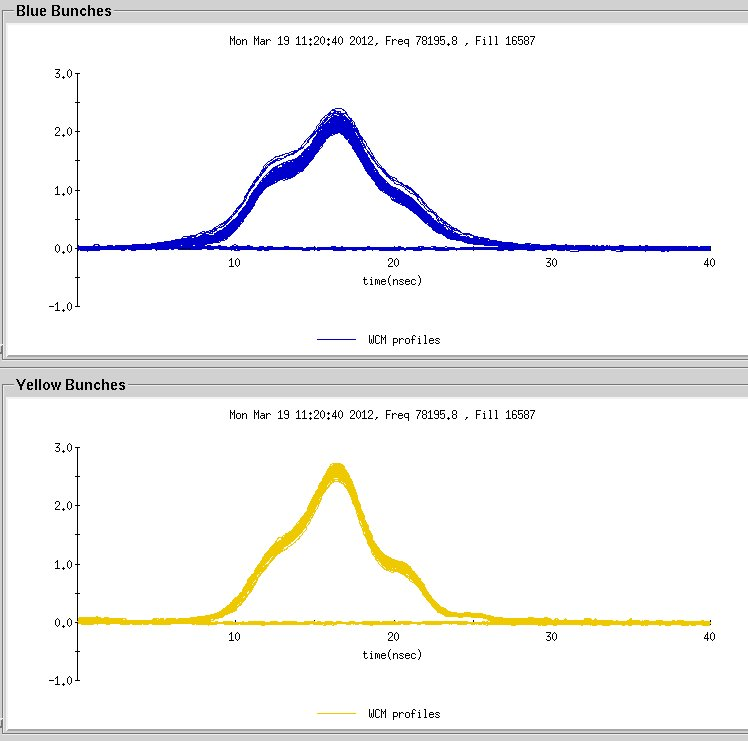
\includegraphics[width=0.7\linewidth]{figures/wcm_16587.jpeg}
  \caption{
    Plot courtesy of Angelika Drees, of RHIC's Collider-Accelerator 
    department. The blue beam (blue) and yellow beam (yellow) are overlaid over
    a 40 nanosecond time period. Even with bunches crossing a fixed point over
    40 nanoseconds, this still corresponds to an overall bunch length of about
    12 meters. Conversely, the bunch width is quite narrow - with Gaussian
    geometry, it is between 150 millimeters and 300 millimeters depending on the
    beam energy. Understanding the beam bunch geometry is a crucial component to
    understanding total the total luminosity delivered by RHIC to PHENIX.
  }
  \label{fig:bunch_profile_overlay}
\end{figure}

\section{Production of Polarized Proton Beams}

The production of polarized beams is a multistage process, and involves
primarily XXX number of experimental components. The importance of polarizing
the beams is fully realized once polarized beams are collided at relatively high
center of mass energies - where the beams behave less like polarized proton
beams, but more like polarized beams of quarks and gluons \cite{Alekseev2003}.
Beam polarization is achieved incrementally - with polarization starting as soon
as the booster and AGS stage of the acceleration process \ref{fig:rhic_complex}.


\section{The Pioneering High Energy Nuclear Interaction Experiment}
\label{sec:PHENIX}
\subsection{Overview}
\subsection{The Spin Program}
\label{sec:beam_polarization}
\subsection{Detector Subsystems}
\subsection{Beam Luminosity at PHENIX}
\subsection{Beam Polarization at PHENIX}
\section{The Forward Upgrade} 
\label{sec:forward_upgrade}

\subsection{The Muon Tracker + Muon Trigger Subsystems}
\subsection{Resistive Plate Chambers}
\subsubsection{Design}
\subsubsection{Construction}
\subsubsection{Testing}
\subsubsection{Performance}
\subsection{Triggering and Data Acquisition}
\subsubsection{2013 Data Set Triggers}
